%% selective-gaussian-blur-body.tex
\paragraph{Beschreibung des Filters aus Nutzersicht}
\glqq Im Gegensatz zu den anderen Weichzeichnungsfiltern wirkt der Selektive Gaußsche Weichzeichner nicht auf alle Pixel des Bildes, der Auswahl oder der aktuellen Ebene. Das Filter wirkt nur auf die Pixel, deren Farbe höchstens um einen definierten Wert von der Farbe der Nachbarpixel abweicht. Daher werden Kanten im Bild erhalten.\glqq\footnote{\url{http://docs.gimp.org/	de/plug-in-sel-gauss.html}} 

Das Filter hat zwei Parameter: 
\begin{itemize}
\item \emph{Blur Radius} - beeinflusst maßgeblich die Intensität der Wirkung. Der Radius wird in Pixeln angegeben.
\item \emph{Max. Delta} - stellt die maximale Farbdifferenz im Bereich von 0 bis 255 pro Farbkanal dar. Dieser Wert beeinflusst maßgeblich, wie gut Kanten
gegen das Weichzeichnen geschützt werden.
\end{itemize}


\paragraph{Algorithmus} 
\begin{algorithm}[h]
\caption{Pseudo-Code des \glqq Selective Gaussian Blur\grqq-Algorithmus}
\label{algo:sel-gaussian}
\begin{algorithmic}[1]

\ForAll{$rows$ $\in input$}
	\ForAll{$columns$ $\in input$}
	\ForAll{$color$ $channels$}
		\State $col\_sum \gets 0$
		\ForAll{$y \in blur\_area$}
			\If{$y$ $\not \in input$}
			\State continue
			\EndIf
			\State $row\_sum \gets 0$
			\ForAll{$x \in blur\_area$}
				\If{$x$ $\not \in input$}
				\State{continue}
				\EndIf
				\State{$diff \gets src\_value - area\_value$}
				\If{$diff < delta$}
				\State{continue}
				\EndIf
				\State{$row\_sum \gets coeff * area\_value$}
			\EndFor
			\State{$col\_sum \gets coeff * row\_sum$}
		\EndFor
		\State $dst\_value \gets col\_sum$
	\EndFor
	\EndFor
\EndFor	
\end{algorithmic}
\end{algorithm}

Der Algorithmus funktioniert pixelweise. Jeder Ausgangspixel wird separat bearbeitet, für jeden Pixel werden Werte für Farbkanäle einzeln berechnet. Bei der Berechnung werden benachbarte Pixelwerte mit einer Faltungsmatrix multipliziert, was in Abbildung \ref{fig:sgb-grid} dargestellt ist. Die Faltungsmatrix ist 2 * \emph{Radius} groß. Bei der Multiplikation wird jedes benachbarte Pixel mit dem zentralen Eingangspixel verglichen, und wenn die Farbdifferenz kleiner als \emph{Max. Delta} ist, trägt dieses Pixel zum Endergebnis bei. 

Der Quellcode hat zwei äußere Schleife, die über die Zeilen und Spalten iterieren. Dann wird pro Farbkanal den Pixelwert berechnet, wo man die Eingangswerte mit den Filterkernwerten multipliziert. Die Multiplikation selbst hat auch zwei Schleifen, die über den Filterkern iterieren.   


\begin{figure}
\centering
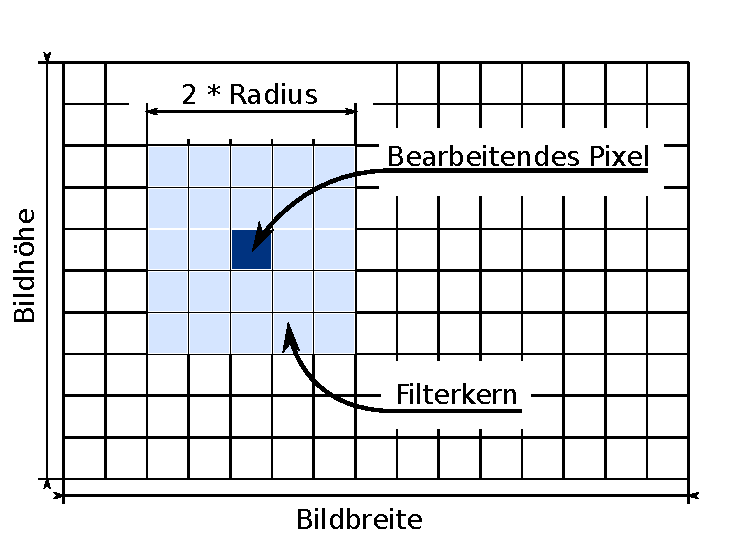
\includegraphics[scale=0.9]{sgb-grid.pdf}
\caption{Selective Gaussian Blur. Schematische Darstellung}
\label{fig:sgb-grid}
\end{figure} 
%Beschreibung Algorithmus allgemeinsprachlich, 
%Pseudocode, visuell
\paragraph{Portierung}
\paragraph{Parallelisierung}
\subparagraph{OpenMP}